% pdfpc Seminar_Presentation.pdf -d 30 --disable-auto-grouping --notes=bottom
\iftrue
\documentclass[compress,11pt,aspectratio=169]{beamer}
\else
\documentclass[compress,11pt,aspectratio=169,notes]{beamer}

\setbeameroption{show notes on second screen=bottom}
\setbeamerfont{note page}{size=\normalsize}
\setbeamertemplate{note page}{
    \pagecolor{black}
    \setlength{\leftmargini}{0pt}
    \setbeamercolor{itemize item}{fg=white}
    \setbeamercolor{normal text}{fg=white}
    \usebeamercolor*{normal text}
    \insertnote
}
\fi

% language and encodings
\usepackage[utf8]{inputenc}
\usepackage[ngerman]{babel}
\usepackage[T1]{fontenc}

% TikZ
\usepackage{tikz}
\usetikzlibrary{positioning}
\usetikzlibrary{shapes.misc}

% other packages
\usepackage{graphicx}               % Bilder einbinden, Version fuer normales latex
\usepackage{ifthen}                 % Zum Auskommentieren von Textteilen
\usepackage{amssymb}                % Mathematische Buchstaben
\usepackage{amsmath}                % Verbesserter Formelsatz
\usepackage{booktabs}               % schönere Tabellen
\usepackage{color}
\usepackage{hyperref}
\hypersetup{urlcolor=black,citecolor=black}
\usepackage{dsfont}
\usepackage{float}
\usepackage{listings}

% \usepackage[style=authoryear,
%             autocite=footnote,
            % backend=biber,
%             giveninits=true]{biblatex}
\usepackage{csquotes}

\usepackage{diagbox}
\usepackage{pgfplots}
\pgfplotsset{compat=1.18}

% \bibliography{biblio.bib}


% Theme
\iffalse
    \usetheme{Singapore}

    \setlength{\leftmargini}{0pt}
    \setbeamersize{text margin left=7.5mm,text margin right=7.5mm}
    
    \setbeamertemplate{section in toc}[sections numbered]
    %\setbeamertemplate{subsection in toc}[subsections numbered]
\else
    % Beamer theme - options:
    % - navigationDotsLocation: specify location of the dots in the headline
    %   - near: display the dots near the section names (default)
    %   - below: display the dots below the section names
    % - titlePageSpacing: vertical spacing between items on title page (default: 1.5em)
    % - titlePageNumberOfAuthors: influence size and location of authors on title page
    %   - few (default): use larger font size, display authors on the left
    %   - many: use smaller font size, display authors on the right
    % - thanksPageBigGraphicsScale: scale for the big graphics on the thanks page (default: 1)
    % - titlePageUniversityLogo: location of university logo file on the title page
    %   (default: logos/logo_us_white)
    % - titlePageInstituteLogo: location of institute logo file on the title page - if empty, nothing is displayed
    %   (default: empty)
    % - titlePageDepartmentLogo: location of department logo file on the title page - if empty, nothing is displayed
    %   (default: empty)
    % - titlePageBigLogo: location of big logo file on the title page - if empty, nothing is displayed
    %   (default: empty)
    % - thanksPageBigGraphics: location of the big graphics on the thanks page
    %   (default: tikz/title)
    % - thanksPageInstituteLogo: location of institute logo file on the thanks page - if empty, nothing is displayed
    %   (default: empty)
    % - thanksPageDepartmentLogo: location of department logo file on the thanks page - if empty, nothing is displayed
    %   (default: empty)
    % - thanksPageBigLogo: location of big logo file on the thanks page - if empty, nothing is displayed
    %   (default: empty)
    \usetheme[
        titlePageUniversityLogo=logos/unistuttgart_logo_deutsch_cmyk_invertiert.png,
        thanksPageBigGraphicsScale=0.175,
        thanksPageBigGraphics=logos/C++_logo.png,
%        thanksPageBigGraphics=thanks,
%        titlePageInstituteLogo=logos/logo_ipvs.png,
%        titlePageDepartmentLogo=logos/logo_sgs.png,
%        titlePageBigLogo=logos/logo_simtech.png,
%        thanksPageInstituteLogo=logos/logo_ipvs.png,
%        thanksPageDepartmentLogo=logos/logo_sgs.png,
%        thanksPageBigLogo=logos/logo_simtech.png,
        navigationDotsLocation=below,
        %titlePageSpacing=0.6em,
        titlePageNumberOfAuthors=many,
    ]{Stuttgart}
\fi

\def\myverzeichnis{.}
\numberwithin{equation}{section}

\hyphenation{}

\title{Selecting the `i'th smallest of `n' elements}
\subtitle{with the fewest possible comparisons.}
\author{von Smercek,~\\Dörrer, Gendle, Steding, Hofmann}
\institute{{\bf Betreuer:} Florian Stober} % TODO: oder FMI - University of Stuttgart?
\date{26. Juni 2023}

\begin{document}
\only<beamer>{\titleframe}

\author{SEA 2025 \hspace{1cm} Johanna Betz}
\section{Introduction}

\sub{1}{0}
\begin{frame}{The Selection Problem}
  \framesubtitle{Finding the $i$-th Smallest Element}
  \uncover<1->{\textbf{Selection($n,i$):} Find the $i$-th smallest element in a collection of $n$ distinct values.}

  \vspace{5mm}

  \centering
  \uncover<2->{Common approaches are based on sorting or partitioning:}

  \vspace{5mm}
  \begin{columns}[T]
    \begin{column}{0.45\textwidth}
      \centering
      \uncover<3->{
        \textbf{Sorting}\\
        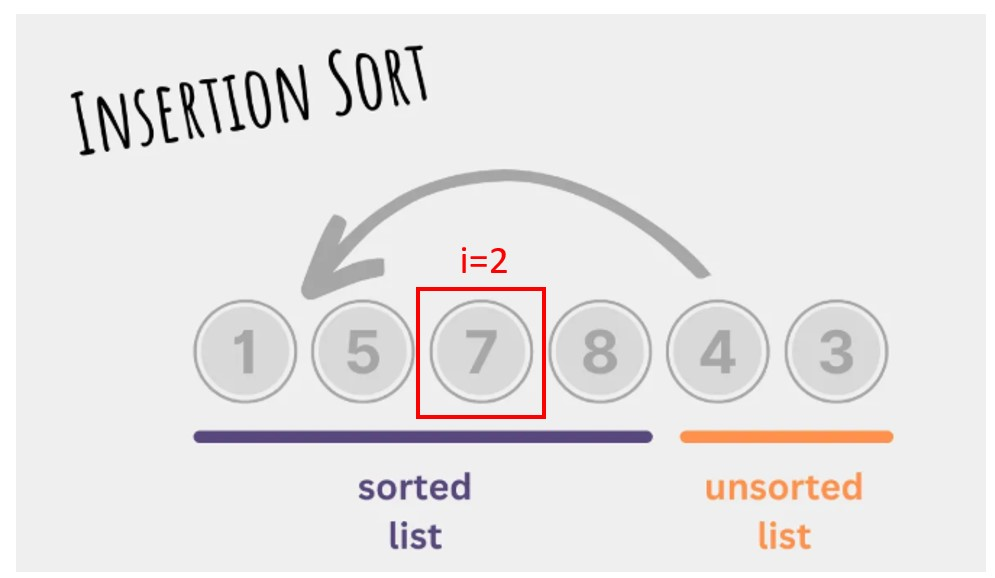
\includegraphics[width=0.8\textwidth, trim={0 0 0 3.5cm}, clip]{figures/Insertion_sort.jpg}\\
        \tiny{Source: medium.com/@teamtechsis}
      }
    \end{column}
    \begin{column}{0.45\textwidth}
      \centering
      \uncover<4->{
        \textbf{Pivoting}\\
        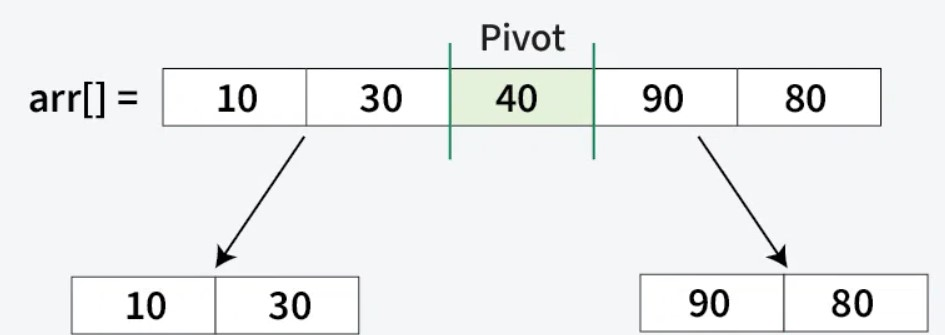
\includegraphics[width=0.8\textwidth]{figures/Pivot.jpg}\\
        \tiny{Source: geeksforgeeks.org}
      }
    \end{column}
  \end{columns}

  \timenote{
    \begin{itemize}
      \item First of all, what is the Selection Problem?
      \item It can be defined by the task of finding the $i$-th smallest element in a collection of $n$ distinct values.
      \item All baseline algorithms either rely on the principle of sorting or pivoting.
      \item I suppose you are familiar with the bubble sort algorithm or insertion sort. With sorting the list first and then just picking the $i$-th element, the selection problem can be solved in a trivial way.
      \item However, this is not the most efficient way, since sorting is in the complexity class of $\mathcal{O}(n log n)$
      \item With pivoting, on the other hand, one can leverage the advantages of divide-and-conquer and apply the well-known Quickselect algorithm or the median of medians appraoch.
      \item \textbf{Let's now look at a more extensive summary of known complexity bounds.}
    \end{itemize}
  }
\end{frame}

\sub{1}{0}
\begin{frame}{Complexity of the Selection Problem}
  \framesubtitle{Known Asymptotic Bounds}
  \begin{itemize}
    \item<+-> Let $V_i^n$ be the worst-case number of comparisons for an optimal algorithm.
    \item<+-> Selecting the minimum is simple: $V_1^n= n-1$.
    \item<+-> The best-known upper bound for selecting the median is $\approx 2.95n$ (Dor and Zwick).
    \item<+-> The proven lower bound for the median is $\approx 2n$ (Bent and John).
    \item<+-> A conjectured lower bound for the median is $\approx 2.41n$ (Schönhage et al.).
  \end{itemize}
  \timenote{
    \begin{itemize}
      \item First of all, let $V_i^n$ be the worst-case number of comparisons for an optimal algorithm.
      \item The easisest case is selecting the minimum.
      \item That is just takes $n-1$ comparisons.
      \item The hardest element to determine is the median.
      \item For this problem, the best-known upper bound is $\approx 2.95n$ comparisons.
      \item The assumed lower bound for the median is $\approx 2.41n$ comparisons.
      \item \textbf{Let's visualize that.}
    \end{itemize}
  }
\end{frame}

\sub{1}{0}
\begin{frame}{Complexity of the Selection Problem}
  \setlength{\abovecaptionskip}{-1pt}
  \begin{figure}
    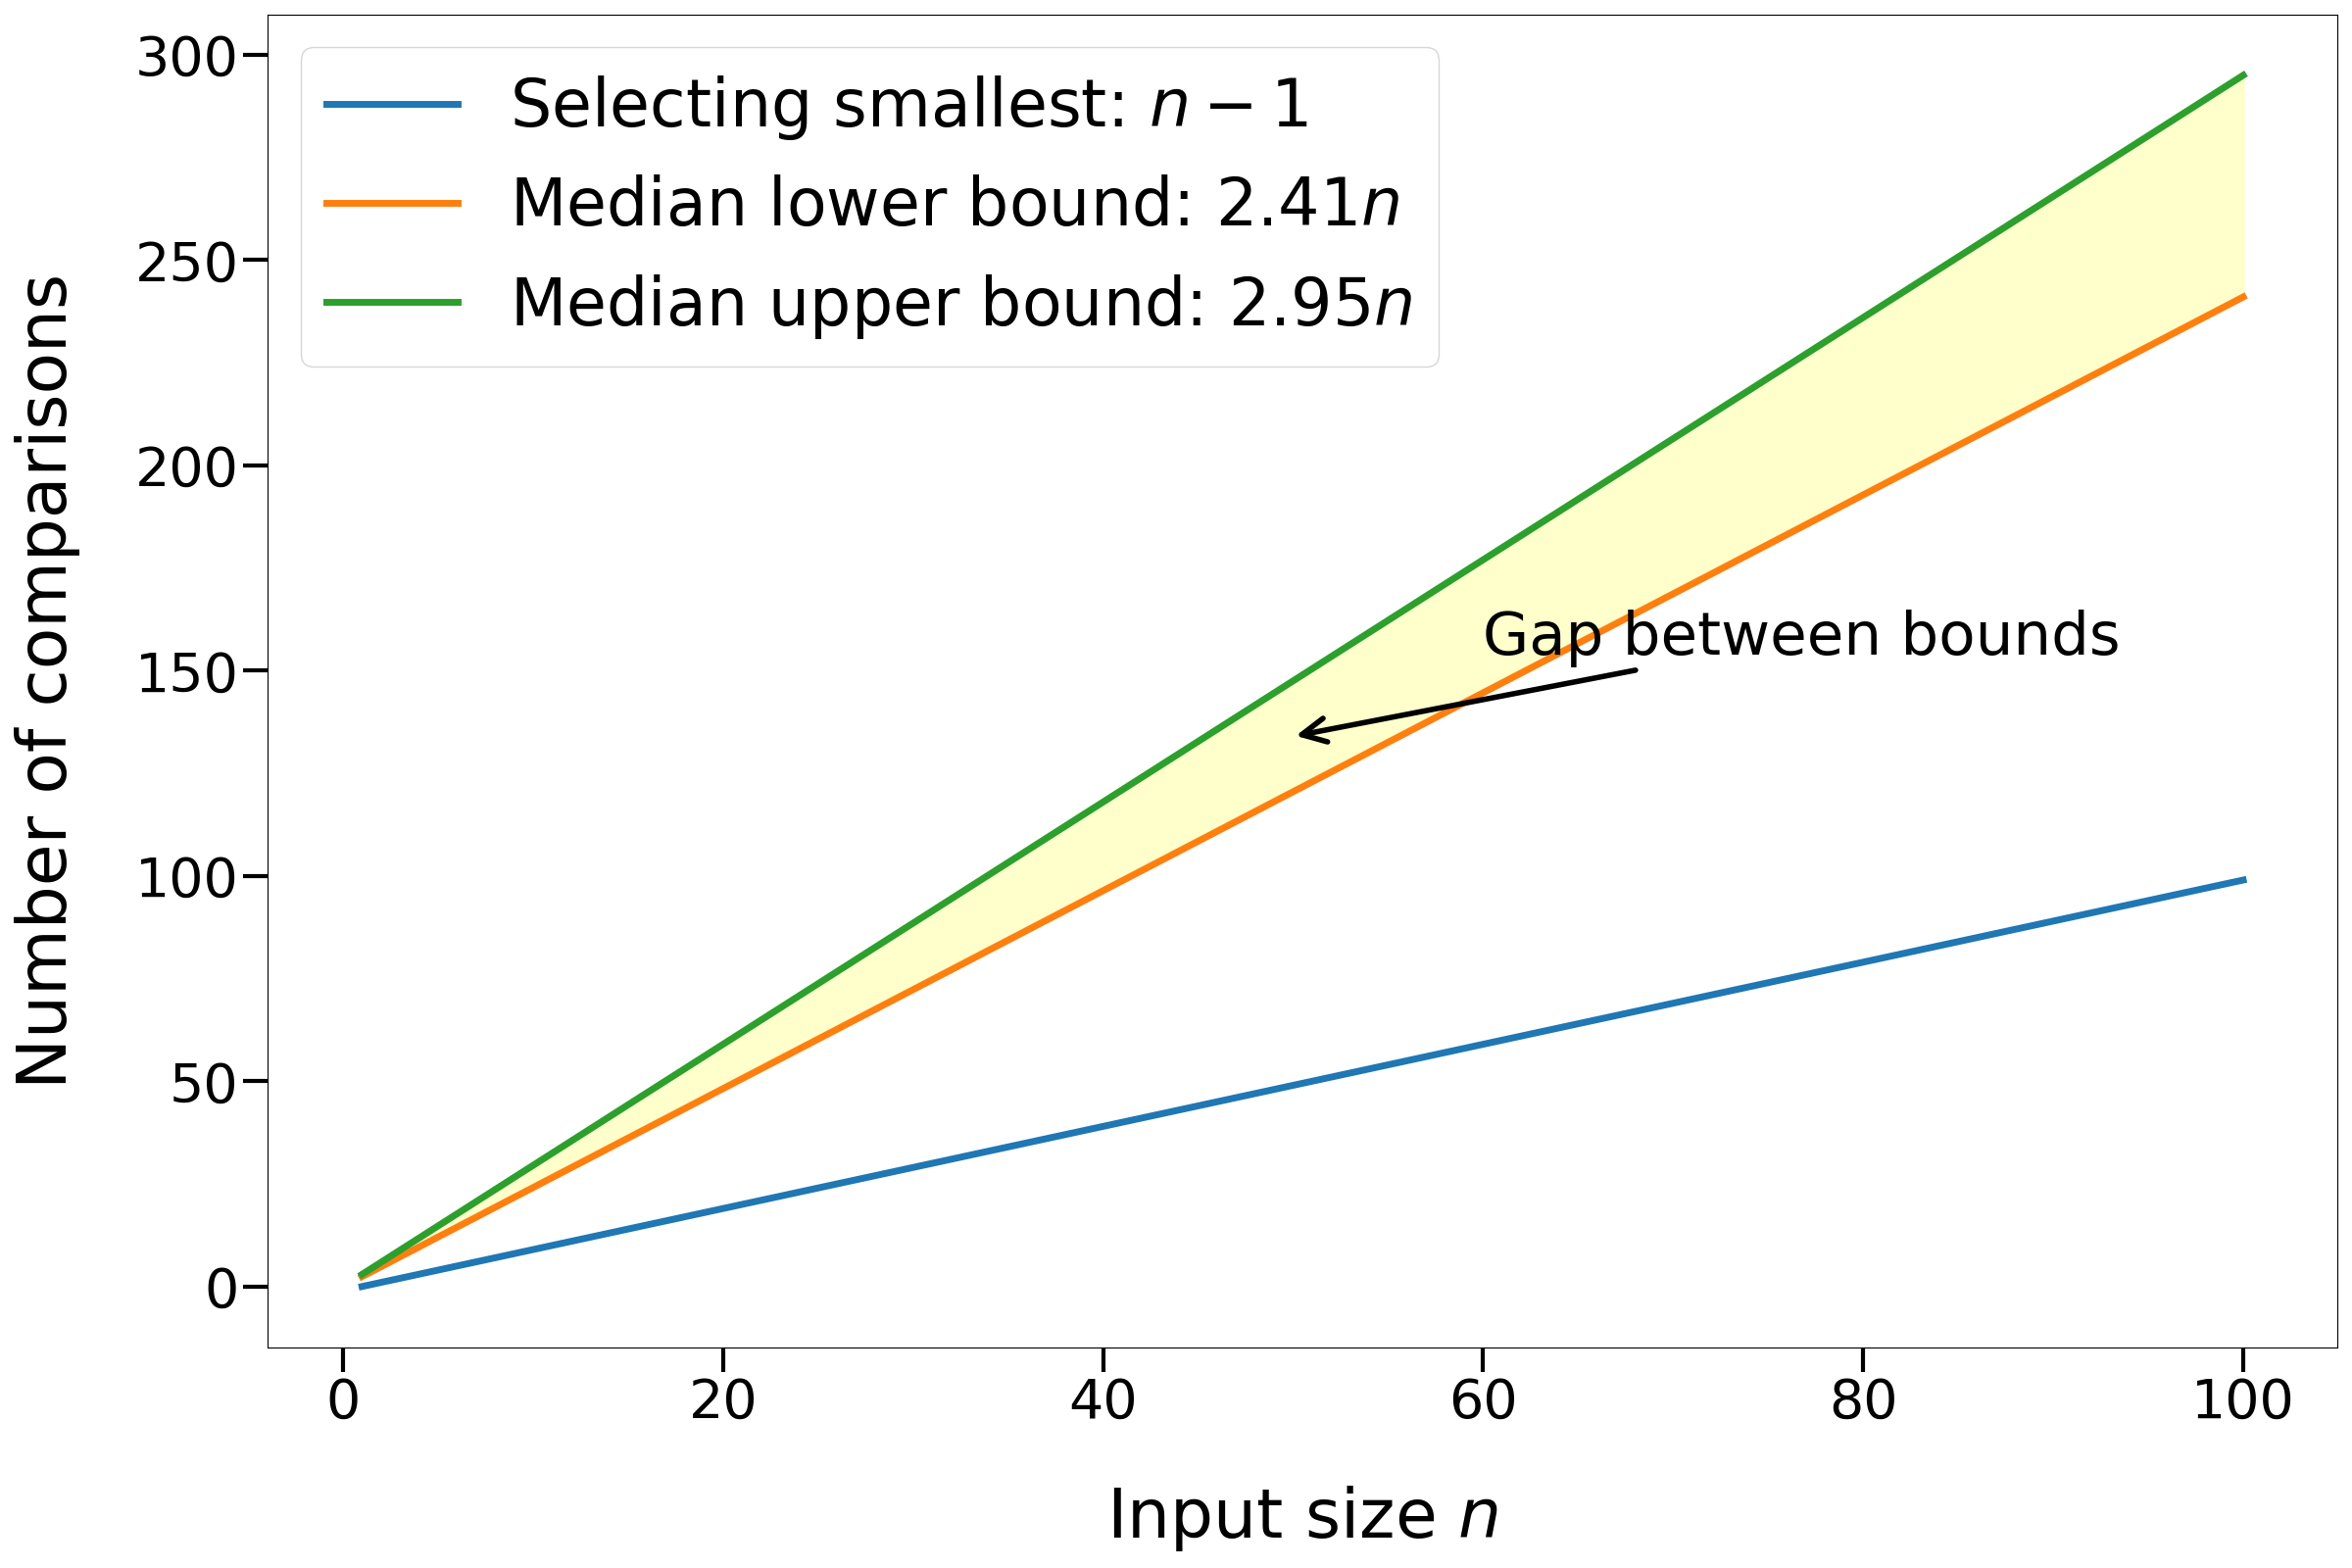
\includegraphics[height=0.7\textheight]{figures/bounds_diagram.png}
    \caption{\small Complexity Bounds for the Selection Problem}
  \end{figure}
  \timenote{
    \begin{itemize}
      \item The green line represents for the numer of comaparions for selecting the smallest element
      \item The orange line represents the lower bound for the median
      \item The blue line represents the upper bound for the median
      \item As can be seen there is a significant gap between selecting the smallest element and the median.
      \item But also between the upper and bound for the median.
      \item With our approach we aim at establishing lower bounds for exact values for $n$ and $i$
      \item This lays ground for elaborating the thightness of the bounds for the median.
      \item And also gives an idea where values for arbitrary $i$ are located in the orange spectrum.
      \item \textbf{This can be summarized by our research question:}
    \end{itemize}
  }
\end{frame}

\sub{1}{0}
\begin{frame}{Complexity of the Selection Problem}
  \begin{figure}
    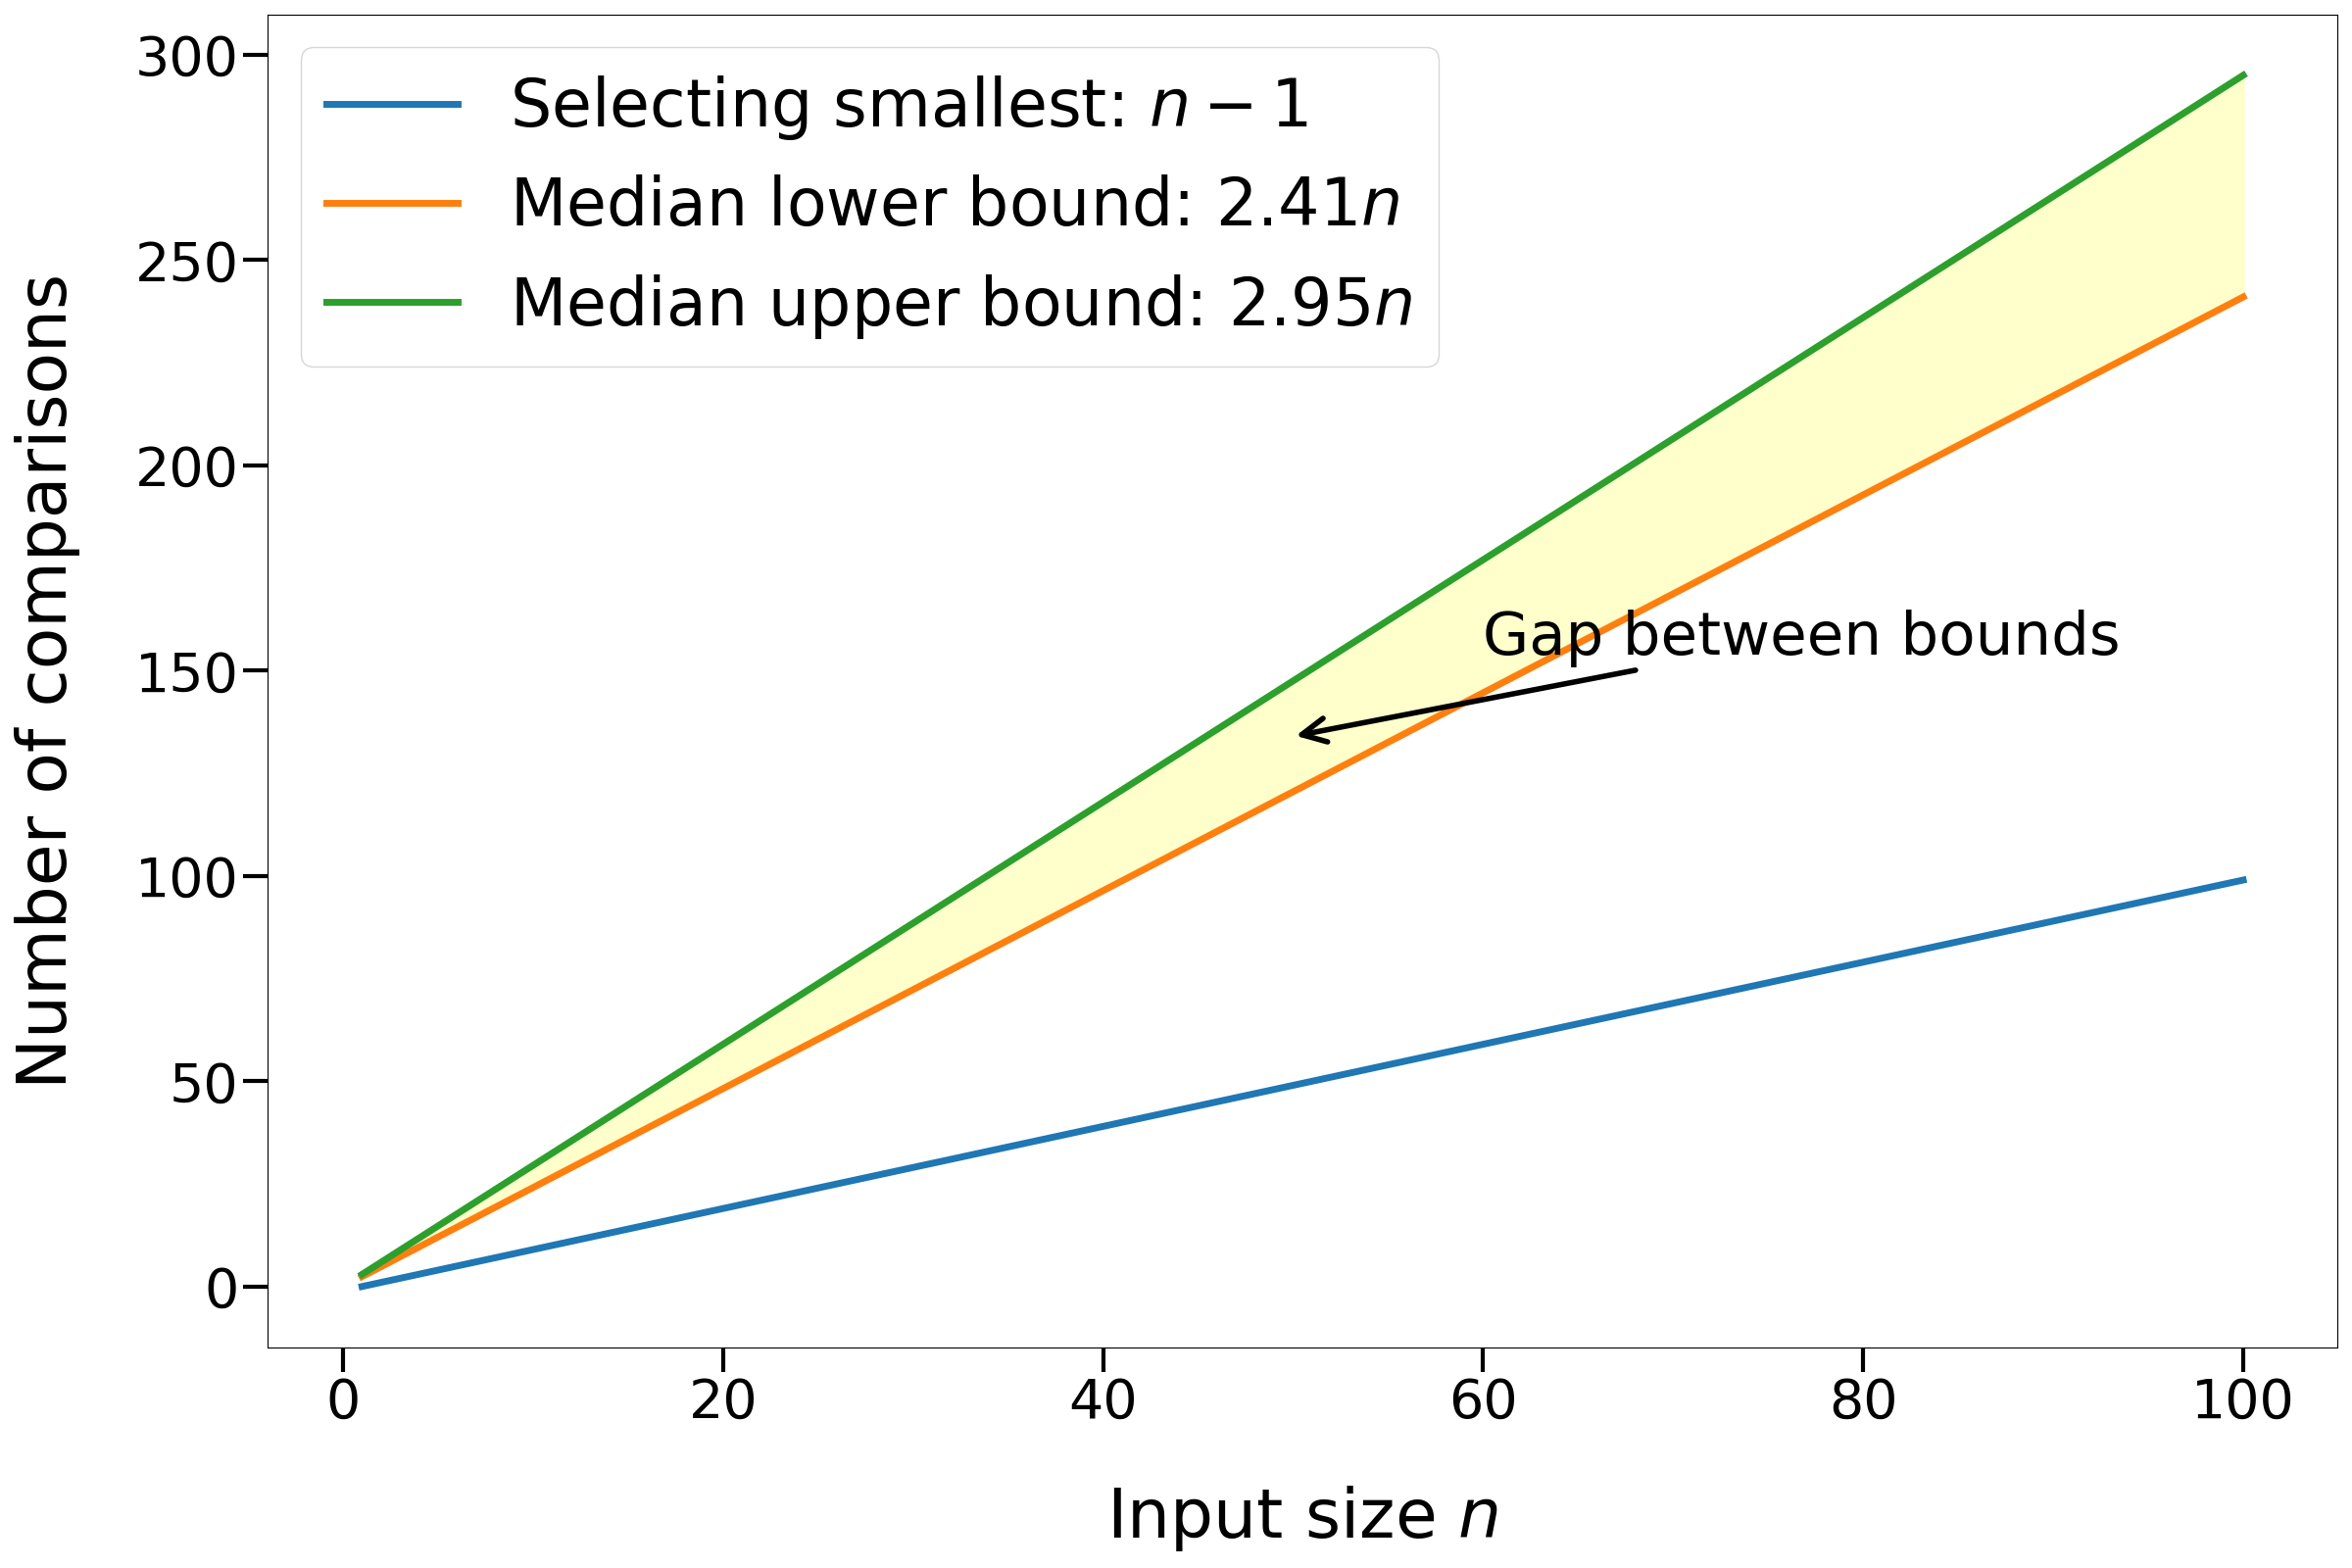
\includegraphics[height=0.5\textheight]{figures/bounds_diagram.png}
    \caption{\small Complexity Bounds for the Selection Problem}
  \end{figure}
  \textbf{Our Question:} What are the \textit{exact} values of $V_i^n$ for small $n$ and arbitrary $i$, and how do they compare to asymptotic bounds?
  \timenote{
    \begin{itemize}
      \item What are the \textit{exact} values of $V_i^n$ for small $n$ and arbitrary $i$, and how do they compare to the asymptotic bounds?
      \item Asymptotic analysis, provide useful insights into the growth behavior of a problem.
      \item However, with automatic analysis one can obtain lower bounds for exact $n$ and $i$.
      \item \textbf{Let's look at some previous work that used automatic analysis for this purpose.}
    \end{itemize}
  }
\end{frame}

\sub{1}{0}
\begin{frame}{Previous Work on Exact Bounds}
  \begin{tabular}{|p{6cm}|p{6cm}|}
    \hline
    \multicolumn{1}{|c|}{Gasarch, Kelly and Puth (1996)}                                               & \multicolumn{1}{c|}{Oksanen (2002)} \\
    \cline{1-2}
    \raggedright \begin{itemize}
                   \item [...]were the first to apply computer search to find lower bounds for the selection problem.
                 \end{itemize} &
    \begin{itemize}
      \item[...] published a computer search algorithm that continues the work of Gasarch et al. for larger $n$ and $i$
    \end{itemize}                         \\
    \cline{1-2}
  \end{tabular}
  \timenote{\footnotesize{
    \begin{itemize}
      \item Gasarch, Kelly and Puth were the first to apply computer search to find lower bounds for the selection problem.
      \item A few years later Oksanen published a computer search algorithm that obtained results for larger $n$ and $i$.
      \item Results are available on his website, but have not been published in any scientific outlet.
      \item This lack of scientific documentation led us to revisit the problem ourselves.
      \item Just to clarify, computer search means that one builds a search tree with all possible comparisons. 
      \item That way one can determine exact lower bounds.
      \item Both previous works build and search the tree in a forward manner, so starting from the root.
      \item We reimplemented the forward search and improve upon it by introducing suitable heuristics.
      \item Additionally we performed backward search, which provides further significant improvements.
      \item \textbf{I will start with Forward Search and Julius will continue with the very interesting backward search.}
    \end{itemize}}
  }
\end{frame}

\section{Forward Search}
\sectionframe{\insertsection}

\begin{frame}{\insertsection: A Minimax Approach}
  \centering
  \begin{tikzpicture}
    [
      level 1/.style = {sibling distance = 4cm},
      level 2/.style = {sibling distance = 2.5cm},
    ]

    \node[anchor=east] at (-7,0) {Min};
    \node[anchor=east] at (-7,-1.5) {Max};
    \node[anchor=east] at (-7,-3) {Min};
    \node[anchor=east] at (-7,-4.5) {Max};

    \node[] (root) {$(n,i,\emptyset)$}
    child {
        node[] {$\{a,b\}$}
        child {
            node[] {$(n,i,\{(a,b)\})$}
            child[sibling distance = 1cm] {
                node[] {$\{c,d\}$}
                child[sibling distance = 1cm] { node[] {$\cdots$}}
                child[sibling distance = 1cm] { node[] {$\cdots$}}
              }
            child[sibling distance = 1cm] { node[] {$\cdots$}}
          }
        child {
            node[] {$(n,i,\{(b,a)\})$}
            child[sibling distance = 1cm] {
                node[] {$\{c,d\}$}
                child[sibling distance = 1cm] { node[] {$\cdots$}}
                child[sibling distance = 1cm] { node[] {$\cdots$}}
              }
            child[sibling distance = 1cm] { node[] {$\cdots$}}
          }
      }
    child {
        node {$\{a,c\}$}
        child[sibling distance = 1cm] { node[] {$\cdots$}}
        child[sibling distance = 1cm] { node[] {$\cdots$}}
      }
    child {
        node[] {$\cdots$}
      }
    ;

    \node[anchor=north east] at (7, -2) {
      \parbox{5.5cm}{
        \begin{itemize}
          \item<2-> \textbf{Depth-first search}
          \item<3-> \textbf{Maximum depth} is limited by one less than the current best result
          \item<4-> \textbf{Optimal algorithm} is build by recording the comparisons that led to the cheapest solution
        \end{itemize}
      }
    };

  \end{tikzpicture}
  \timenote{\footnotesize
    \begin{itemize}
      \item \textbf{The forward search starts at the root with the initial problem instance} which consists of the $n$, the $i$ and an empty set. This set will be filled with all relations resulting from the comparisons.
      \item In the following it will also be called partially ordered set or short poset.
      \item On the next level, pairs of elements are formed.
      \item Each pair has two child nodes representing both possible outcomes of the comparison.
      \item With a minimax approach, the optimal number of comparisons in the worst case is obtained.
      \item The max nodes cosinder the worst case outcome of the comparison 
      \item The min nodes, however, consider the most intelligent comparison of all pairs.
      \item The search tree is traversed using a depth-first search. This saves memory and enables pruning.
      \item We limit the maximum number of comparisons assigned to child problems is limited to one less than the current best result.
      \item The search program builds algorithms by recording, for each problem, the comparison that led to the cheapest result.
    \end{itemize} }
\end{frame}

\sub{1}{0}
\begin{frame}{Optimizations}
  \begin{columns}
    \begin{column}{0.6\textwidth}
      \begin{itemize}
        \item<1-> \textbf{Iterative deepening}
        \item<2-> \textbf{Reduce posets} by removing all elements that cannot be the i-th smallest
        \item<3-> \textbf{Approximated canonical representation} based on a hash of
          \begin{itemize}
            \item in- and out-degree
            \item hash of adjacent vertices
          \end{itemize}
        \item<4-> \textbf{Cache} previous results and the currently known minimum for unsolvable posets.
      \end{itemize}
    \end{column}

    \begin{column}{0.4\textwidth}
      \uncover<2->{%
        \vspace{1cm} % Adjust this value to shift the graphic upward
        \begin{tikzpicture}
          \draw(0.5, -5.5) rectangle (5.2, -2.9);
          \node[circle,draw=black] (C1) at (1, -5.0) {};
          \node[circle,draw=black] (C2) at (1, -4.0) {};
          \node[circle,draw=black] (C3) at (2, -3.5) {};
          \node[cross out, line width=1pt, draw=red] at (2, -3.5) {}; % red cross overlay
          \node[circle,draw=black] (C4) at (2, -4.5) {};
          \node[circle,draw=black] (C5) at (3, -4.5) {};

          \draw (C1) -- (C2);
          \draw (C3) -- (C4);
          \draw (C2) -- (C3);

          \node[draw=none] at (4, -3.5) {\footnotesize $n=5, i=3$};
        \end{tikzpicture}
      }
    \end{column}
  \end{columns}
  \timenote{
    \small
    \begin{itemize}
      \item Let's now look at some of the optimizations we applied.
      \item We use iterative deepening, which means that the number of allowed comparisons is increased after each tree traversal.
      \item We work on reduced posets. For each poset, we remove elements that cannot be the i-th smallest. If an element has $i$ or more elements that are smaller or more than $n-i$ elements larger, it is removed.
      \item We compute an approximated canonical representation of the problem based on a hash value
      \item This hash value is computed for the sink and all other nodes iteratively, based on their in and out-degrees and the hash of the adjacent nodes.
      \item Doing so a few times yields a pretty good approximation of an canonical representation that can be used for isomorphic testing.
      \item Furthermore, we cache previous results meaning whether a poset is solvable or not.
      \item In the case of not solvable we additionally store the currently known lower bound.
      \item Besides simple reuse purposes, the information in the cache can be used for pruning by cutting off branches that contradict the minimum value in the cache.
      \item \textbf{Speaking of pruning. Let's look at two further pruning techniques we developed.}
    \end{itemize}
  }
\end{frame}

\sub{1}{0}
\begin{frame}{Pruning techniques}
  \framesubtitle{\large Compatible solutions}
  \uncover<1->{The solved problem $(S,i)$ is a \textbf{compatible solution} of the problem $(R,i)$, if
    \begin{align*}
      a <_S b \Rightarrow b \not <_R a
    \end{align*}}
  \vspace*{0.5mm}

  \uncover<2->{Denote the \textbf{number of compatible solutions} with $\vert \mathcal{C}(P,i) \vert $}
  \vspace{5mm}

  \raggedright
  \hspace*{-3mm}
  \uncover<3->{\begin{tabular}{l p{10cm}}
      \textbf{Lemma: } & Selecting the $i$-th smallest element of a poset $P$ requires at least $\lceil log (|C(P, i)|) \rceil $ comparisons
    \end{tabular}}
  \timenote{\begin{itemize}
      \item The first one I would like to talk about leverages the concept of compatible solution.
      \item We say a solved problem is a compatible solution of another problem if there are no contradicting relations.
      \item We denote the \textbf{number} of compatible solutions with the absolute of C(P,i)
      \item The useful lemma related to compatible solutions is the following:
      \item Selecting the i-th smallest element of a poset $P$ requires at least $\lceil log (|C(P, i)|) \rceil $ comparisons
      \item The reasoning behind this...
      \item
    \end{itemize}}
\end{frame}

\sub{1}{0}
\begin{frame}{Pruning techniques}
  \framesubtitle{\large Compatible solutions}
  \only<1>{
    \begin{tikzpicture}
      [
        level 1/.style = {sibling distance = 4cm},
        level 2/.style = {sibling distance = 3cm},
        level 3/.style = {level distance=1.2cm}
      ]

      \node[anchor=east] at (-7,0) {Min};
      \node[anchor=east] at (-7,-1.5) {Max};
      \node[anchor=east] at (-7,-3) {Min};
      \node[anchor=east] at (-7,-4.2) {Max};

      \node[] (root) {$(n,i,\emptyset)$}
      child {
          node[] {$\{a,b\}$}
          child {
              node[] {$(n,i,\{(a,b)\})$}
              child[sibling distance = 1cm] {
                  node[] {$\{c,d\}$}
                  child[sibling distance = 1cm] { node[] {$\cdots$}}
                  child[sibling distance = 1cm] { node[] {$\cdots$}}
                }
              child[sibling distance = 1cm] { node[] {$\cdots$}}
            }
          child {
              node[] {$(n,i,\color{red}\underbrace{\{(b,a)\}}_{=P}\color{black})$}
              child[sibling distance = 1cm] {
                  node[] {\color{black}$\{c,d\}$}
                  child[sibling distance = 1cm] { node[] {$\cdots$}}
                  child[sibling distance = 1cm] { node[] {$\cdots$}}
                }
              child[sibling distance = 1cm] { node[] {$\cdots$}}
            }
        }
      child {
          node {$\cdots$}
        }
      child {
          node[] {$\cdots$}
        }
      ;


    \end{tikzpicture}
  }
  \only<2>{
    \begin{tikzpicture}
      [
        level 1/.style = {sibling distance = 4cm},
        level 2/.style = {sibling distance = 3cm},
        level 3/.style = {level distance=1.2cm}
      ]

      \node[anchor=east] at (-7,0) {Min};
      \node[anchor=east] at (-7,-1.5) {Max};
      \node[anchor=east] at (-7,-3) {Min};
      \node[anchor=east] at (-7,-4.2) {Max};

      \node[] (root) {$(n,i,\emptyset)$}
      child {
          node[] {$\{a,b\}$}
          child {
              node[] {$(n,i,\{(a,b)\})$}
              child[sibling distance = 1cm] {
                  node[] {$\{c,d\}$}
                  child[sibling distance = 1cm] { node[] {$\cdots$}}
                  child[sibling distance = 1cm] { node[] {$\cdots$}}
                }
              child[sibling distance = 1cm] { node[] {$\cdots$}}
            }
          child {
              node[] {$(n,i,\color{red}{\underbrace{\{(b,a)\}}_{=P}}\color{black})$}
              child[sibling distance = 1cm] {
                  node[] {\color{black}$\{c,d\}$}
                  child[sibling distance = 1cm] { node[] {$\cdots$}}
                  child[sibling distance = 1cm] { node[] {$\cdots$}}
                }
              child[sibling distance = 1cm] { node[] {$\cdots$}}
            }
        }
      child {
          node {$\cdots$}
        }
      child {
          node[] {$\cdots$}
        }
      ;

      \draw[red] (-3.8,-1.8) -- (-3.1,-2.3);
      \draw[red] (-3.8,-2.3) -- (-3.1,-1.8);

      \node [draw=none] at (1.2, -2.05) {\color{red} If $\lceil \log (\vert \mathcal{C}(P,i)\vert ) \rceil > $ remaining comparisons allowed};


    \end{tikzpicture}
  }

  \timenote{
    \begin{itemize}
      \item Let's now look at a small example for pruning based on compatible solutions.
    \end{itemize}
  }
\end{frame}

\sub{1}{0}
\begin{frame}{Pruning techniques}
  \framesubtitle{\large Free comparison}
  \begin{columns}
    \begin{column}{0.65\textwidth}
      \begin{itemize}
        \item<1-> Already applied by Oksanen
        \item<2-> Add a useful relation between a large element and a small element
          %\item<3-> Search for unrelated elements $a$ and $b$ such that $a$ has at least two smaller elements and $b$ has at least two smaller elements
        \item<3-> allows more extensive poset reduction
        \item<4-> allows for pruning because, if problem with the free comparison is not solvable, then so is the original problem
      \end{itemize}
    \end{column}
    \begin{column}{0.35\textwidth}
      \uncover<3->{\begin{figure}
          \begin{tikzpicture}[node distance=1.2cm]
            \node[draw, circle, minimum size=0.5cm] (1) {b};
            \node[draw, circle, minimum size=0.5cm, below right of=1] (2) {};
            \node[draw, circle, minimum size=0.5cm, below left of=1] (3) {};

            \node[draw, circle, minimum size=0.5cm, above of=1, node distance=1.5cm] (4) {a};
            \node[draw, circle, minimum size=0.5cm, above right of=4] (5) {};
            \node[draw, circle, minimum size=0.5cm, above left of=4] (6) {};

            \path[dashed] (1) edge (4);

            \path[-]
            (1) edge (2)
            (1) edge (3)
            (4) edge (5)
            (4) edge (6);
          \end{tikzpicture}
        \end{figure}}
    \end{column}
  \end{columns}
\end{frame}

\author{SEA 2025 \hspace{1cm} Julius von Smercek}

\section{Backward Search}
\sectionframe{\insertsection}
\timenote{
  \LARGE
  Thank you! Now I would like to continue with the backward search.
}

\sub{1}{44}
\begin{frame}<1-5>{\insertsection}
  Start with a solved poset and search the empty poset
  \vfill
  \begin{itemize}
    \item<+-> \textbf{Goal:} Given an upper bound $k$, find all posets solvable in at most $k$ comparisons.
    \item<+-> \textbf{Initialization:} Start with the set of all posets that are already ``solved'' (i.e., the $i$-th element is uniquely identified). Their cost is 0.
    \item<+-> \textbf{Canonization:} A unique normal form (with `nauty`) is expensive, but required. We use fast invariants to pre-filter, such that `nauty` is needed for only $< 0.1\%$ of posets.
    \item<+-> \textbf{Iteration (Level $k \to k+1$):} To find all posets solvable in $k+1$ steps, find all \textit{predecessors} of posets solvable in $\leq k$ steps.
    \item<+-> \textbf{Termination:} The search stops when the initial empty poset $(n, i, \emptyset)$ is generated. Its level is the value $V_i^n$.
  \end{itemize}
  \timenote{
    \LARGE
    \only<1>{
      In contrast to the forward search, the backward search starts with a solved poset and seeks to find the empty poset with $n$ elements.

      For this, an iterative deepening approach is employed.
      For a given upper bound $k$, this approach finds all posets that can be solved in a maximum of $k$ comparisons.
    }
    \only<2>{
      To achieve this, we start with the set of posets that are already solved, meaning the $i$-th element is uniquely identifiable.
      The cost for each poset in this set is $0$, as they can be solved in $0$ comparisons.

      To avoid redundant computations, we use a normal form that reduces the set of solved posets to a single one: the poset containing only one element for which the minimum is obvious.
      It should be evident that this poset can be solved directly.
    }
    \only<3>{
      This unique normal form is based on leveraging duality and `nauty`.
      While computationally expensive, `nauty` is necessary to guarantee a unique normal form.
      Although an approximate normal form was sufficient for the forward search, a unique normal form is essential for the correctness of the backward search.
      Consequently, we have combined `nauty` with our own procedure, reducing the usage of `nauty` to less than $0.1\%$ of cases.
    }
    \only<4>{
      In each iteration level, we compute all posets that are solvable in $k+1$ steps, given that we know the set of all posets solvable in fewer than $k$ steps.
      To do this, we compute the predecessors of all posets from the previous level.
      I will elaborate on the precise definition of a predecessor shortly.
    }
    \only<5>{
      The search terminates when the empty poset is found.
      The level in which the empty poset with the desired $n$ and $i$ first appears corresponds to the optimal number of comparisons required.
    }
  }
\end{frame}

\sub{0}{50}
\begin{frame}<1-4>{Predecessor Computation}
  \begin{definition}[Predecessor]
    Suppose the set of all posets solvable in $k$ comparisons is known.
    A normalized poset $Q$ is a \textbf{predecessor} iff there exists a comparison between two elements $u,v$ such that
    \begin{enumerate}
      \item<2-> Adding the relation $(u,v)$ to $Q$ yields a known poset solvable in exact $k$ steps
      \item<2-> Adding the relation $(v,u)$ to $Q$ yields a known poset solvable in at maximum $k$ steps
      \item<3-> $Q$ itself was not found at a lower level
    \end{enumerate}
  \end{definition}
  \vfill
  \visible<4>{
    This process essentially ``removes'' a comparison to go one step backward.
  }
  \timenote{
    \LARGE
    \only<1>{
      Okay, let's now define the concept of a predecessor.

      A predecessor is determined by removing a comparison. For this, we assume that the set of all posets solvable in k comparisons is known. This set is therefore a given.
    }
    \only<2>{
      A normalized poset Q is then considered a predecessor if there exists a comparison between two elements, u and v, such that adding the relation (u, v) to Q results in a known poset that is solvable in exactly k steps, and adding the relation (v, u) results in a known poset that is solvable in at most k steps.
    }
    \only<3>{
      This ensures that regardless of the outcome of the comparison, Q is solvable in exactly $k + 1$ comparisons. And, obviously, Q must not have been discovered yet.
    }
    \only<4>{
      This process essentially removes one comparison.
    }
  }
\end{frame}

\sub{1}{16}
\begin{frame}<1-4>{Example}
  \vspace{-0.75cm}
  \begin{figure}[!b]
    \centering
    \scalebox{0.8}{\begin{tikzpicture}

  % Level k = 4
  \uncover<1-3>{
    \node at (-1, 8) {$k=\text{ ?}$};
  }
  \uncover<4->{
    \node at (-1, 8) {$k=4$};
  }

  \node[circle,fill=black,scale=0.5] (k4_1) at (2.125 + 0 * 0.75, 8) {};
  \node[circle,fill=black,scale=0.5] (k4_2) at (2.125 + 1 * 0.75, 8) {};
  \node[circle,fill=black,scale=0.5] (k4_3) at (2.125 + 2 * 0.75, 8) {};
  \node[circle,fill=black,scale=0.5] (k4_4) at (2.125 + 3 * 0.75, 8) {};
  \node at (2.125 + 0.75 * 1.5, 7.5) {$i=2$};

  \uncover<4->{
    \draw[->, dashed] (4, 7.25) -- (4.5, 6.75);
    \draw[->] (3.75, 7.25) -- (4.25, 6.75);

    \draw (-1, 7) -- (6.5, 7);

    % Level k = 3
    \node at (-1, 6.25) {$k=3$};

    \node[circle,fill=black,scale=0.5] (k3_1) at (1 + 0 * 0.75, 6.25) {};
    \node[circle,fill=black,scale=0.5] (k3_2) at (1 + 1 * 0.75, 6.25) {};
    \node[circle,fill=black,scale=0.5] (k3_3) at (1 + 2 * 0.75, 6.25) {};
    \node at (1 + 0.75, 5.75) {$i=2$};

    \draw[->, dashed] (2.5, 5.5) -- (3, 5);
    \draw[->] (2.25, 5.5) -- (2.75, 5);

    \node[circle,fill=black,scale=0.5] (k3_4) at (4 + 0 * 0.75, 6.5) {};
    \node[circle,fill=black,scale=0.5] (k3_5) at (4 + 0 * 0.75, 6) {};
    \node[circle,fill=black,scale=0.5] (k3_6) at (4 + 1 * 0.75, 6.25) {};
    \node[circle,fill=black,scale=0.5] (k3_7) at (4 + 2 * 0.75, 6.25) {};
    \draw (k3_4) -- (k3_5);
    \node at (4 + 0.75, 5.75) {$i=2$};

    \draw[->, dashed] (5, 5.5) -- (5.25, 5);
    \draw[->] (4.75, 5.5) -- (5, 5);
  } \uncover<3->{

    \draw (-1, 5.25) -- (6.5, 5.25);

    % Level k = 2
    \node at (-1, 4.25) {$k=2$};

    \node[circle,fill=black,scale=0.5] (k2_1) at (0 + 0 * 0.75, 4.5) {};
    \node[circle,fill=black,scale=0.5] (k2_2) at (0 + 1 * 0.75, 4.5) {};
    \node[circle,fill=black,scale=0.5] (k2_3) at (0 + 2 * 0.75, 4.5) {};
    \node at (0 + 0.75, 4) {$i=1$};

    \draw[->, dashed] (1.5, 3.75) -- (2.5, 2.75);
    \draw[->] (1.25, 3.75) -- (2.25, 2.75);

    \node[circle,fill=black,scale=0.5] (k2_4) at (3 + 0 * 0.75, 4.25) {};
    \node[circle,fill=black,scale=0.5] (k2_5) at (3 + 0 * 0.75, 4.75) {};
    \node[circle,fill=black,scale=0.5] (k2_6) at (3 + 1 * 0.75, 4.5) {};
    \draw (k2_4) -- (k2_5);
    \node at (3 + 0.75 * 0.5, 3.75) {$i=2$};

    \draw[->, dashed] (3.375, 3.5) .. controls (4.25, 2.75) .. (3.5, 1.5);
    \draw[->] (3.125, 3.5) -- (3.125, 2.75);

    \node[circle,fill=black,scale=0.5] (k2_7) at (5.25 + 0 * 0.75, 4.25) {};
    \node[circle,fill=black,scale=0.5] (k2_8) at (5.25 + 0 * 0.75, 4.75) {};
    \node[circle,fill=black,scale=0.5] (k2_9) at (5.25 + 1 * 0.75, 4.25) {};
    \node[circle,fill=black,scale=0.5] (k2_10) at (5.25 + 1 * 0.75, 4.75) {};
    \draw (k2_7) -- (k2_8);
    \draw (k2_9) -- (k2_10);
    \node at (5.25 + 0.75 * 0.5, 3.75) {$i=2$};

    \draw[->, dashed] (4.75, 3.5) -- (4, 3);
    \draw[->] (5, 3.5) -- (4.25, 3);
  } \uncover<2->{

    \draw (-1, 3.25) -- (6.5, 3.25);
    % Level k = 1
    \node at (-1, 2.5) {$k=1$};

    \node[circle,fill=black,scale=0.5] (k1_1) at (2.875 + 0 * 0.75, 2.75) {};
    \node[circle,fill=black,scale=0.5] (k1_2) at (2.875 + 1 * 0.75, 2.75) {};
    \node at (2.875 + 0.75 * 0.5, 2.25) {$i=1$};

    \draw[->, dashed] (3.375, 2) -- (3.375, 1.5);
    \draw[->] (3.125, 2) -- (3.125, 1.5);
  }

  \draw (-1, 1.75) -- (6.5, 1.75);

  % Level k = 0
  \node at (-1, 1) {$k=0$};

  \node[circle,fill=black,scale=0.5] (k0_1) at (3.25, 1.25) {};
  \node at (3.25, 0.75) {$i=1$};
\end{tikzpicture}
}
    \caption{Search tree for $n=4,i=2$}
    \label{fig:backward-searchtree-bound4}
  \end{figure}

  \timenote{
    \Large
    \only<1>{
      I've brought an example to illustrate this.

      We start with the solved poset at the bottom and are looking for the second smallest element in an empty poset with four elements. Obviously, the solved poset is solved in 0 comparisons; for the initial poset at the top, the number of comparisons is still unknown.
    }
    \only<2>{
      The very first thing we do is compute all posets that are solvable in one comparison. In this case, there is only one poset with two elements for which we are searching the minimum. Theoretically, the dual of this poset - that is, the poset with two elements where we seek the maximum - would also be on this level, but since they are isomorphic, one can be omitted.

      The solid arrow here represents the resulting poset if the comparison (u, v) were to be inserted, and the dashed lines represent the resulting poset if the opposite comparison were inserted.
    }
    \only<3>{
      Analogously, we can compute the level for $k = 2$. Here you can see it nicely again: the solid arrow always points to the level directly below it, while the other arrow points to some level further down.
    }
    \only<4>{
      In this way, we can construct the tree until we finally find a path from the empty poset to the solved poset at $k = 4$. This means that this subtree represents an optimal algorithm for finding the second smallest element among four elements.
    }
  }
\end{frame}

\sub{0}{44}
\begin{frame}<1-3>{Removing Comparisons}
  \begin{figure}[!b]
    \centering
    \scalebox{1.5}{\begin{tikzpicture}
  \node[circle,draw=black] (A1) at (0, 0) {};
  \node[circle,draw=black] (A2) at (0, 1) {};
  \node[circle,draw=black] (A3) at (0, 2) {};

  \draw (A1) -- (A2) node {};
  \draw (A2) -- (A3) node {};
  \node (AL) at (0, -0.5) {$i = 1$};
  \node (A) at (0, -1) {(1)};


  \node[circle,draw=black] (B1) at (2.5 + 0, 0) {};
  \node[circle,draw=black] (B2) at (2.5 + 0, 2) {};
  \node[circle,draw=black] (B3) at (2.5 + 1, 1) {};

  \draw (B1) -- (B2) node {};
  \node (BL) at (2.5 + 0.5, -0.5) {$i = 1$};
  \node (B) at (2.5 + 0.5, -1) {(2)};


  \node[circle,draw=black] (C1) at (5 + 1, 2) {};
  \node[circle,draw=black] (C2) at (5 + 0, 0) {};
  \node[circle,draw=black] (C3) at (5 + 2, 0) {};

  \draw (C1) -- (C2) node {};
  \draw (C1) -- (C3) node {};
  \node (CL) at (5 + 1, -0.5) {$i = 1$};
  \node (C) at (5 + 1, -1) {(3)};
\end{tikzpicture}}
    \caption{Ambiguous result of removing a comparison due to transitivity}
    \label{fig:backward-problematic-case}
  \end{figure}
  \timenote{
    \LARGE
    \only<1>{
      A problem that may already be apparent here is that the removal of comparisons is not unambiguous.
      We are given a poset with three elements, where we know that the bottom element is less than the middle one, and the middle element is less than the top one.
      This edge is invisible in the Hasse diagram.
    }
    \only<2>{
      If we now remove the red comparison between the bottom and the middle element, it is possible that the transitive edge between the top and bottom elements remains.
    }
    \only<3>{
      Consequently, if the transitive edge does not exist, the middle poset could be the result.
      However, if the edge still exists, then the last case would apply.
      The fact that removing a single comparison can lead to multiple possible posets complicates the problem.
    }
  }
\end{frame}

\sub{0}{28}
\begin{frame}{Poset Distribution}
  \begin{figure}[!b]
    \centering
    \resizebox{0.9\textheight}{!}{%
      \begin{tikzpicture}
  \begin{axis}[
      ymode=log,
      axis x line = bottom,%x-Achse nur unten
      % x dir=reverse,
      enlarge x limits = .05,%x-Achse erweitern
      x axis line style = {-},%kein Pfeil
      % title = {\dots},
      ylabel={Number of posets},
      xlabel={Number of comparisons removed},
      % only marks,
      cycle list={{mark=x}},
      legend pos=north east,
    ]
    \addlegendentry{$i = 1$}
    \addplot+[cyan] table { %n=14,i=0
        x  y
        0  1
        1  1
        2  1
        3  1
        4  1
        5  1
        6  1
        7  1
        8  1
        9  1
        10 1
        11 1
        12 1
        13 1
      };
    \addlegendentry{$i = 2$}
    \addplot+[green] table { %n=14,i=1
        x y
        0  1
        1  1
        2  3
        3  6
        4  11
        5  21
        6  41
        7  61
        8  59
        9  42
        10 28
        11 19
        12 12
        13 7
        14 4
        15 2
        16 1
      };
    \addlegendentry{$i = 3$}
    \addplot+[magenta] table { %n=14,i=2
        x y
        0  1
        1  1
        2  3
        3  14
        4  60
        5  287
        6  1385
        7  4005
        8  5510
        9  4268
        10 2284
        11 1025
        12 428
        13 180
        14 73
        15 30
        16 11
        17 6
        18 2
        19 1
      };
    \addlegendentry{$i = 4$}
    \addplot+[orange] table { %n=14,i=3
        x y
        0  1
        1  1
        2  3
        3  16
        4  175
        5  2201
        6  22900
        7  103210
        8  191627
        9  174416
        10 94785
        11 37004
        12 12173
        13 3851
        14 1211
        15 392
        16 124
        17 41
        18 13
        19 4
        20 2
        21 1
      };
    \addlegendentry{$i = 5$}
    \addplot+[yellow] table { %n=14,i=4
        x y
        0  1
        1  1
        2  3
        3  16
        4  323
        5  10111
        6  200521
        7  1386176
        8  3607272
        9  4267576
        10 2763862
        11 1162696
        12 367875
        13 100552
        14 26024
        15 6745
        16 1781
        17 474
        18 127
        19 34
        20 12
        21 4
        22 1
        23 1
      };
    \addlegendentry{$i = 6$}
    \addplot+[red] table { %n=14,i=5
        x y
        0  1
        1  1
        2  3
        3  16
        4  446
        5  26921
        6  780123
        7  6588569
        8  19882832
        9  26416869
        10 18631911
        11 8243306
        12 2630332
        13 688904
        14 164372
        15 38334
        16 8918
        17 2084
        18 518
        19 130
        20 36
        21 11
        22 4
        23 1
        24 1
      };
    \addlegendentry{$i = 7$}
    \addplot+[blue] table { % n=14,i=6
        x y
        0  1
        1  1
        2  3
        3  16
        4  452
        5  37236
        6  1389385
        7  14591680
        8  53003482
        9  82198656
        10 65707713
        11 31909980
        12 10770689
        13 2864659
        14 665109
        15 147573
        16 32349
        17 7214
        18 1624
        19 400
        20 100
        21 27
        22 9
        23 4
        24 1
        25 1
      };
  \end{axis}
\end{tikzpicture}
    }
    \caption{Number of posets for $n = 14$ depending on the number of comparisons}
  \end{figure}
  \timenote{
    \LARGE
    Another interesting aspect is the poset distribution for the backward search.
    Here, we have plotted the number of removed comparisons against the number of found posets on a logarithmic scale for different values of $i$.
    It is noticeable that for larger $i$, significantly more posets must be searched.
    Another interesting point is that the peak of searched posets for all $i$ lies between 5 and 10, which will also present a challenge for the bidirectional search.
  }
\end{frame}


\section{Results}
\sectionframe{\insertsection}

\sub{0}{33}
\begin{frame}{Exact Bounds}
  \vspace{-1cm}
  \begin{table}[!t]
    \label{tab:results}
    \centering
    \small
    \begin{tabular}{c|cccccccc}
      $n$ & \multicolumn{8}{c}{$i$}                                                                                                      \\
          & 1                       & 2  & 3           & 4           & 5           & 6           & 7                 & 8                 \\ \hline
      1   & 0                                                                                                                            \\
      2   & 1                                                                                                                            \\
      3   & 2                       & 3                                                                                                  \\
      4   & 3                       & 4                                                                                                  \\
      5   & 4                       & 6  & 6                                                                                             \\
      6   & 5                       & 7  & 8                                                                                             \\
      7   & 6                       & 8  & 10          & 10                                                                              \\
      8   & 7                       & 9  & 11          & 12                                                                              \\
      9   & 8                       & 11 & 12          & 14          & 14                                                                \\
      10  & 9                       & 12 & 14          & 15          & 16                                                                \\
      11  & 10                      & 13 & 15          & 17          & 18          & 18                                                  \\
      12  & 11                      & 14 & 17          & 18          & 19          & 20                                                  \\
      13  & 12                      & 15 & 18          & 20          & 21          & 22          & 23                                    \\
      14  & 13                      & 16 & 19          & 21          & 23          & 24          & \textbf{25}                           \\
      15  & 14                      & 17 & 20          & 23          & \textbf{24} & \textbf{26} & \textbf{26}       & \textbf{27}       \\
      16  & 15                      & 18 & \textbf{21} & \textbf{24} & \textbf{26} & \textbf{27} & \textbf{28} -- 33 & \textbf{28} -- 36 \\
    \end{tabular}
  \end{table}
  \timenote{
    \LARGE
    Let us first, however, turn to the results.
    In the presented table, all values that we have newly computed are shown in bold.
    We have, of course, verified all other values.
    In doing so, we were able to improve an existing lower bound, specifically for $n = 15, i = 5$, and prove that the correct lower bound is 24 comparisons.
    For the values $i = 7$ and $8$ at $n = 16$, we could not determine the exact number of comparisons, but we were able to establish a new lower bound.
  }
\end{frame}

\sub{1}{01}
\begin{frame}<1-5>{Contribution}
  \definecolor{counterexample}{rgb}{0.8, 0.1, 0.1}
  \setbeamercolor{block title alerted}{bg=gray!20,fg=black}
  \setbeamercolor{block body alerted}{bg=gray!5}
  \begin{itemize}
    \item<+-> Verified existing results and generated executable algorithms
    \item<+-> Calculated and corrected new lower bounds
    \item<+-> Introduced compatible posets and backward search as novelty for this problem
    \item<+-> Disproved a conjecture on optimal algorithm structure from Gasarch:
      ``An optimal algorithm exists that first compares all elements pairwise.''
      \begin{alertblock}<+->{Counterexample: $n=12, i=5$}
        The conjecture implies a minimum of 20 comparisons are required. \\[0.5em]
        \textbf{Our discovered algorithm succeeds with only \textcolor{counterexample}{19} comparisons.}
      \end{alertblock}
  \end{itemize}
  \timenote{
    \LARGE
    \only<1>{
      To summarize our contribution, we have verified all previous results and generated executable algorithms with the optimal number of comparisons in Rust.
    }
    \only<2>{
      Furthermore, we contribute the new lower bounds as well as the improved value for $n = 15$.
    }
    \only<3>{
      A key component is also the backward search, which was used for the first time for this problem, as well as heuristics, such as the compatible posets, which had not been applied to this problem before.
    }
    \only<4>{
      Finally, we were able to refute a conjecture by Knuth, which was already mentioned as a comment in Oksanen's C program, but could be definitively disproven by our program due to the partial incorrectness of the C code.
    }
    \only<5>{
      He conjectured that an optimal algorithm exists which first compares all elements pairwise.
      We found a counterexample for this, namely for $n=12, i=5$.
      With this assumption, the optimal algorithm requires $20$ comparisons, which does not correspond to the optimal bound of $19$ comparisons.
    }
  }
\end{frame}

\sub{0}{51}
\begin{frame}{Runtime Comparison}
  \begin{table}[!t]
    \label{tab:times}
    \renewcommand{\arraystretch}{1.0}
    \centering
    \resizebox{1.0\textheight}{!}{%
      \begin{tabular}{c|c|l|l|l}
        $n$ & $i$ & \textbf{Forward Search} & \textbf{Backward Search} & \textbf{Oksanen}                                         \\
        \hline
        14  & 1   & 0.0s                    & 0.0s                     & 0.0s                                                     \\
        14  & 2   & 0.0s                    & 1.5s                     & 0.0s                                                     \\
        14  & 3   & 1.4s                    & 5.9s                     & \textbf{0.6s}                                            \\
        14  & 4   & \textbf{35.9s}          & 46.9s                    & 1m 47s                                                   \\
        14  & 5   & 17m 27s                 & \textbf{15m 33s}         & 6h 29m                                                   \\
        14  & 6   & 2h 40m                  & \textbf{1h 40m}          & 4d 10h                                                   \\
        14  & 7   & 14h 40m                 & \textbf{6h 27m}          & >5d                                                      \\
        \hline
        15  & 1   & 0.0s                    & 0.0s                     & 0.0s                                                     \\
        15  & 2   & 0.1s                    & 4.0s                     & \textbf{0.0s}                                            \\
        15  & 3   & 2.8s                    & 25.9s                    & \textbf{1.4s}                                            \\
        15  & 4   & \textbf{2m 24s}         & 13m 11s                  & 27m 17s                                                  \\
        15  & 5   & 1h 12m                  & \textbf{45m 52s}         & 1d 5h 40m\footnote{calculates a non-optimal lower bound} \\
        15  & 6   & 1d 8h 37m               & \textbf{19h 30m}         & >5d                                                      \\
        15  & 7   & 4d 23h 37m              & \textbf{1d 5h 43m}       & >5d                                                      \\
        15  & 8   & 14d 1h 51m              & \textbf{3d 8h 9m}        & >5d                                                      \\
      \end{tabular}
    }
  \end{table}
  \timenote{
    \Large
    Finally, it is interesting to see how long we had to heat the university to compute these results.
    An important timenote here is that the forward search is only single-threaded, whereas the backward search is fully parallelized and runs almost linearly faster with the number of threads. With 48 threads and 1 TB of utilized RAM, this makes a significant difference.
    For $n=14$ and $n=15$, I have marked in bold the values that were computed the fastest.
    For very small values, Oksanen's C program is faster; however, for moderate values, the forward search is superior, and for the large values, the backward search is, which is relatively consistent.
    We can see here, for example, that for ($n=15, i=8$), the backward search, taking three days, significantly outperforms the forward search, which would have taken 14 days.
  }
\end{frame}

\sub{1}{00}
\begin{frame}<1-3>{Future Work}
  \vspace{-1.2cm}
  \begin{columns}
    \begin{column}{.49\textwidth}
      \begin{itemize}
        \item<+-> Idea of bidirectional Search: Run forward and backward search simultaneously
        \item<+-> Challenge: The searches intersect only after $> 99.9\%$ of the search space has been explored in both searches
        \item<+-> Forward search can prune subtrees, but the backward search needs to calculate the full tree
      \end{itemize}
    \end{column}
    \begin{column}{.49\textwidth}
      \onslide<2->{
        \begin{figure}[!b]
          \centering
          \renewcommand{\arraystretch}{0.9}
          \resizebox{0.85\textheight}{!}{%
            \begin{tikzpicture}
  \begin{axis}[
      ybar,
      ymode=log,
      axis x line = bottom,%x-Achse nur unten
      enlarge x limits = .1,%x-Achse erweitern
      x axis line style = {-},%kein Pfeil
      bar width=3pt,
      ylabel={number of posets},
      xlabel={number of comparisons},
      % legend cell align=left,
      % legend pos=outer north east,
      % legend style={at={(0.5,-0.2)},anchor=north}, % draw=none
    ]
    % \addlegendentry{forward search}
    \addplot[fill=blue,shift={(1pt, 0)}] table {
        x y
        0  1
        1  4
        2  57
        3  552
        4  10397
        5  154828
        6  1166640
        7  3770182
        8  5941732
        9  4726819
        10 2096404
        11 604582
        12 143058
        13 32460
        14 7450
        15 1823
        16 471
        17 132
        18 41
        19 13
        20 5
        21 3
        22 2
        23 1
      };
    % \addlegendentry{backward search}
    \addplot[fill=red,shift={(-1pt, 0)}] table {
        x y
        23 1
        22 1
        21 3
        20 16
        19 381
        18 15227
        17 290138
        16 1750707
        15 4058631
        14 4368185
        13 2592437
        12 1006071
        11 291970
        10 72346
        9  16728
        8  3898
        7  893
        6  227
        5  58
        4  17
        3  6
        2  2
        1  1
        0  1
      };
  \end{axis}
\end{tikzpicture}

Treff: 11
          }
          \caption{Poset distribution for $n = 13$, $i = 7$}
          \label{fig:backward_forward_count_13_6}
        \end{figure}
      }
    \end{column}
  \end{columns}
  \timenote{
    \LARGE
    \only<1>{
      For the future, we could imagine parallelizing the forward search or developing even better heuristics.
      A bidirectional search would also be conceivable.
      This means we would start the forward and backward searches simultaneously and solve the problem from both ends.
    }
    \only<2>{
      The problem with this approach is that the intersection point of the two searches is only reached after 99.9 percent of the posets have been searched for both directions.
      We have just seen that in the backward search, the search tree explodes very early, which conversely also happens in the forward search.
      We can see this again in this illustrative graph:
      The number of posets for the forward and backward searches are shown in blue and red, respectively.
    }
    \only<3>{
      A possible idea would be to develop pruning strategies for the backward search, although it unfortunately has to search through almost all posets to guarantee correctness.
      These approaches are currently the subject of ongoing research, with the bidirectional search appearing to be the most promising.
    }
  }
\end{frame}

\sub{0}{06}
\thanksframe

\timenote{
  \LARGE
  On that timenote, I would like to thank you for your attention.
  If you have any questions, we would be happy to answer them now.
}

% % TODO: prevent in toc above

% \sub{0}{04}
% \begin{frame}[shrink=25]{References}
%   \nocite{*}
%   \printbibliography[heading=none]
%   \timenote{
%     \LARGE
%     Here are our references, which can also all be found in our paper.
%   }
% \end{frame}

% \begin{frame}[shrink=25]{Image References}
%   \begin{itemize}
%     \item[] https://medium.com/@teamtechsis/introduction-to-sorting-algorithms-1623b9cdd4f1
%     \item[] https://www.geeksforgeeks.org/dsa/quick-sort-algorithm/
%   \end{itemize}
% \end{frame}

% % TODO: Bildquellen & unser eigenes Paper
\end{document}
